% Implementation (4000 words)
% * Refer to design strategies that looked ahead to the testing stage
% * Draw attention to what is not my own work (ie rebar, webmachine etc)
% * Major milestones might be highlighted with advantage
% *! Show evidence of skill, clear thinking and common sense

% ************
% Should have: 
% 	intro
% 	content
% 	summary
% ************

% Word budget 4000 words. Try to keep it less
\chapter{Implementation}
In this chapter we will go from a high level overview of the components of my system to the more intricate details of how routing differs between Chord and Pastry.
We will also look at Erlang process supervision and how hot code reloading shortened my development time.

\section{Process}
% How use testing throughout to get desired behaviour
The implementation process was very goal oriented. The goals and milestones I had set in my project proposal had been clarified and expanded upon in the pre-development analysis phase and guided me through the implementation phase.

Whenever I found bugs during the development and testing of my system, I would reproduce the bug through failing tests before correcting them. This let me to build up a suite of regression tests adding to my existing set of unit tests.

The Distributed Hash Tables Chord and Pastry being central parts of my design and the main focus of the subsequent evaluation efforts, took the majority of my development time. This will also be reflected by the attention I will give them in this chapter.


\section{High level system components}
% What components does the system consist of?
% Want design that is DHT agnostic
My search engine has two main parts. The search server itself, including the Distributed Hash Tables and supporting components, and a central control hub.

The central control hub served as a system wide dashboard, giving me an overview over the number of machines participating in my search network and how many Distributed Hash Table nodes were being run by each machine along with if they were Pastry or Chord nodes. The central control hub also allowed me to run coordinated experiments across my network.

In figure \ref{figComponents} you see an overview of the components in the software running on the machines that were part of my search network. With small modifications in the controller component, removing parts that are specific to the experimental setup used for my experiments, and some security hardening of the Distributed Hash Table component, the same setup could be used in a final release of my software.

% Component overview
\begin{figure}[!htb]
\begin{center}
	\includegraphics[width=0.9\linewidth]{illustrations/ComponentOverview.eps}
\caption{High level overview of the components of the search application. The arrows show the part a component relies on.}
\label{figComponents}
\end{center}
\end{figure}

In order to be able to use Chord or Pastry interchangeably I had specified a minimalistic API the Distributed Hash Tables should expose to their surroundings. This approach makes it easier to keep the system modular and contain areas of responsibility to the different components.

The arrows in figure \ref{figComponents} show which components a component relies on to provide services for it. The Friend Search Web API exposes the HTTP API to the world and in turn uses the Friend Search server for resolving search queries into link records and then profile records that can be displayed to the end user. The Friend Search server uses the Distributed Hash Tables for finding the records, and the Distributed Hash Tables have local data stores that store the data items the particular Distributed Hash Table node is responsible for.

The controller is the component that interacts directly with the central control hub system and starts and stops Distributed Hash Table nodes. It also regulates if Pastry or Chord nodes should be run.

During experimental runs, the controller is also the component that issues requests to the local Distributed Hash Tables.

The logger is used for logging events during experiments, and is specific to the experimental setup. It would not be included in final deployments of the system.

\subsection{Third party code}
% Which components are not developed by me?
The Friend Search Web API in figure \ref{figComponents} uses an Erlang library called Webmachine in order to handle the HTTP negotiation process correctly. Webmachine in turn relies on another Erlang library called Mochiweb which the Friend Search Web API also uses in order to serialize the search results into JSON for consumption by the clients.

\section{Distributed Hash Tables}
I will now discuss Distributed Hash Tables in more detail. We will first look at the general ideas that Distributed Hash Tables are built upon, before going into detail on how Chord and Pastry perform routing, which is where they differ the most.

\subsection{General idea}
% Design of DHT's
% Distributed Hash Tables
%   Key ideas
Distributed Hash Tables are Hash Tables, in some languages also called dictionaries, where the data is stored across a network of machines. Distributed Hash Tables store data under particular keys, and given a key will return the data stored under it if it exists.

Specific for my implementations is that I used a bag approach where I allow multiple items to be stored under the same key. This is necessary to avoid link records for common name fragments to replace each other.

Distributed Hash Tables differ from regular hash tables in that the different parts of the key-space are stored on different nodes, potentially running on different machines. The node responsible for a given subsection of the key-space stores all values with keys falling into that key segment, and is also subsequently the one asked when the value is retrieved.

The Chord key-space is an integer key-space ranging from 0 up to $2^{160} - 1$. It wraps around at the end such that $2^{160} - 1$ immediately precedes 0. It can be useful to think of the key-space as circular.

The Pastry key-space is likewise an integer key-space. The Pastry paper suggest using keys in the range of 0 up to $2^{128} - 1$, but to increase code reuse between Chord and Pastry I decided to let Pastry use a key space from 0 up to $2^{160} - 1$ as well.

Both Chord and Pastry nodes do themselves also have keys associated with them that lie in the same key-space. The node key in the case of my implementations is the hash of the machines public IP-address and the port number the node is listening to. What is important is that the node keys are evenly distributed in the key-space, because they are also used to split up the key-space.

Chord and Pastry differ in how the key-space is divided between the nodes. While a Chord node is responsible for all keys greater than the key of the node preceding it in the key-space and up to and including its own key-value (figure \ref{figKeyspaceChord}), a node in Pastry is responsible for all keys that are numerically closer to itself than it is to the neighbours on either side of it (figure \ref{figKeyspacePastry}). While the difference doesn't sound dramatic, it, as we will see shortly, very much influences the way in which the routing is performed.

\begin{figure}[!htb]
\begin{center}
	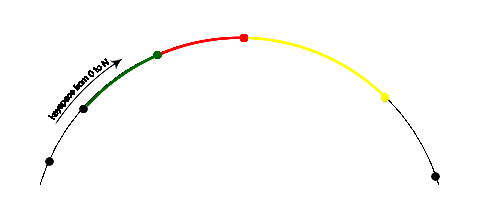
\includegraphics[width=0.9\linewidth]{illustrations/ChordKeySpace.eps}
  \caption{Illustration of how the keyspace is divided between Chord nodes.}
  \label{figKeyspaceChord}
\end{center}
\end{figure}

\begin{figure}[!htb]
\begin{center}
	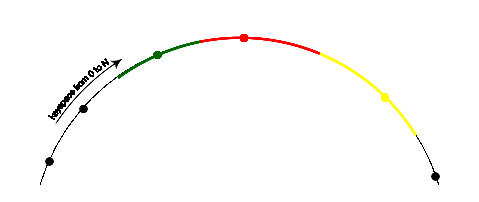
\includegraphics[width=0.9\linewidth]{illustrations/PastryKeySpace.eps}
  \caption{Illustration of how the keyspace is divided between Pastry nodes.}
  \label{figKeyspacePastry}
\end{center}
\end{figure}

Just like in regular hash tables, the performance is best if a good hashing function is used to generate keys, such that the keys are evenly spread in the key-space. This minimizes collisions, and in the case of Distributed Hash Tables also ensures that the machines in the network get roughly equal shares of both the data and the traffic.

\subsection{Routing}
%   What is different between Chord and Pastry?
%   How is routing done?
We will first look at how Chord does its routing, look at my implementation of the core algorithm, and then do the same for Pastry.

I have omitted supporting functions that do not add to the understanding of the routing procedure to keep the source code listings short and to the point.


\paragraph{Routing in Chord}
Each Chord node maintains a routing table with information about other nodes participating in the Distributed Hash Table. It contains more nodes closely succeeding it in the key-space than it does nodes further away. 

If a Chord node wants to lookup a key, it asks the node in its routing table most closely preceding the key if it knows about another node more closely preceding it. If it does, the Chord node looking for the key in turn asks this new node if it knows about a node more closely preceding the target key. Once the node immediately preceding the target key is found, its successor is asked for the value of the key. Figure \ref{figRoutingChord} illustrates this process. Note how the Chord node that is trying to lookup the key is involved in the whole lookup process.

\begin{figure}[!htb]
\begin{center}
	\includegraphics[width=0.9\linewidth]{illustrations/ChordRoutingSuccess.png}
  \caption{This figure shows Chord's approach to routing.}
  \label{figRoutingChord}
\end{center}
\end{figure}

The following code listing shows the Chord function \emph{perform\_find\_successor} which Chord uses internally to find the node succeeding a key. 
It very closely follows the Chord routing procedure as it was explained above. 
First the node in the nodes local routing table that most closely precedes the target key is found (line 4). In illustration in figure \ref{figRoutingChord} this would correspond to node B. This node is then used to find the node most closely preceding the target key. Given the node immediately preceding the key, its successor is returned by the perform\_find\_successor function on line 9.

\lstinputlisting[label=find_successor,caption=Finding the successor of a key]{sourceCode/find_successor.erl}

In code listing \ref{find_predecessor} we see how we use a remote procedure call to ask another node for a node more closely preceding the target key. This process recursively continues until we have found the node directly preceding the target key.
Using the setup in figure \ref{figRoutingChord} as an example, the data returned by the remote procedure call to node B in the first recursion would be respectively D as the next finger, and the node represented as a dot between B and C as the successor. 

\lstinputlisting[label=find_predecessor,caption=Finding the predecessor of a key]{sourceCode/find_predecessor.erl}

The procedure for finding the closest\_preceding\_finger follows below.
It iterates over an array of routing table entries (called finger table entries in the Chord jargon) starting from the node with a key furthest away in the key-space and successively getting closer to its own key. The first node with a key falling between the nodes own key and the target key is returned.

\lstinputlisting[label=closest_preceding_finger,caption=Returns the node most closely preceding the key]{sourceCode/closest_preceding_finger.erl}

The implementation of closest\_preceding\_finger is slightly clumsy because of the edge case where there is no match in the routing table and the node itself should be returned. I therefore ended up with duplicated bound checking logic, that I refactored into the following function. What it does is check if a given finger is the finger we are looking for. If it is not it recursively calls closest\_preceding\_finger to have it process the next finger.

\lstinputlisting[label=check_closest_preceding_finger,caption=Check if a finger is the closest known finger to a key. Returns the node most closely preceding the key]{sourceCode/closest_preceding_finger.erl}


\paragraph{Routing in Pastry}
Much like Chord nodes, nodes in Pastry also maintain routing tables. The Pastry routing table has three different parts. It contains a leaf set of nodes that are a nodes neighbours in terms of the key-space, a list of nodes that are its neighbours in terms of the proximity heuristic, and a table that allows it to look up nodes closer to the target key than itself.

When a Pastry node looks up a key, unlike Chord, it hands over the responsibility of finding the node responsible for the key, to the node it knows about closest to the key. This node in turns passes the responsibility to a node still closer to the key than itself, and this process repeats itself until the target node is found. Contrast figure \ref{figRoutingPastry} showing the Pastry approach of routing to the way Chord performs its routing shown in figure \ref{figRoutingChord}. In the Pastry approach the node initiating the lookup takes no part in the routing after having started it.

\begin{figure}[!htb]
\begin{center}
	\includegraphics[width=0.9\linewidth]{illustrations/PastryRoutingSuccess.png}
  \caption{This figure shows Pastry's approach to routing.}
  \label{figRoutingPastry}
\end{center}
\end{figure}

The following code listings show how this procedure is implemented. Thanks to Erlang's expressive nature, the core routing algorithm, much like in the case of Chord, is nice and compact.

The Pastry routing procedure is organized slightly differently from what it looks like in Chord. In Pastry all inter-node communication is handled by routing messages.
Message can be lookup requests, but also requests to store data for a given key or join a Pastry network.

The following code listing shows the main \emph{route\_msg} function. 
The router first tries to route the message to a node in its leaf set. If that fails it tries to find a match in the routing table on line 4 and falls back to routing to any node in the routing table numerically closer to the key than itself on line 5.

\lstinputlisting[label=route_msg,caption=Routes a message towards a recipient]{sourceCode/route_msg.erl}

In listing \ref{route_to_leaf_set} we see that if the match in the leaf set is the node itself, then the message is delivered to the main pastry application on line 5. Otherwise the message is forwarded to a closer node if appropriate on line 7.

\lstinputlisting[label=route_to_leaf_set,caption=Routes a message to the leaf set if applicable]{sourceCode/route_to_leaf_set.erl}

If routing to the leaf set fails, the node tries routing the message to a node in the routing table sharing more digits in the key with the target key than what itself does. Again, just like when routing to the leaf set, if the best match is itself, the message is delivered.

\lstinputlisting[label=route_to_node_in_routing_table,caption=Routes a message to a node in the routing table if applicable]{sourceCode/route_to_node_in_routing_table.erl}

If all other routing approaches fail, the last resort the Pastry node has is to find any node that is numerically closer to the key than what itself is.

\lstinputlisting[label=route_to_closer_node,caption=Routes a message to any closer node]{sourceCode/route_to_closer_node.erl}

\subsection{Replication of data}
My implementations of Chord and Pastry both replicate data amongst their immediate neighbours for fault tolerance. While this is only proposed as extensions in the Chord and Pastry papers, I thought it worthwhile implementing this functionality.

\mbox{}

This concludes my discussion of the implementation of Chord and Pastry. We have seen how Distributed Hash Tables operate with circular integer key-spaces and how routing was implemented in Chord and Pastry.

\section{Search server}
% Search server
The search server is what glues together the client facing HTTP API and the Distributed Hash Tables. It receives the search queries from the clients, converts them into appropriate keys that it can lookup in the Distributed Hash Tables, and resolves link records it gets returned to full profile records that can be shown as search results.

The current implementation is rather na\"ive, and while it does basic ranking of results, prioritising what it predicts are better matches, it performs no caching of results which would significantly improve the performance.

\section{Central control hub}
% Hub control server
% Focus on testing and evaluation
The central control hub is a service that runs under a domain name known by all the search engine nodes.
When the friend search client application is started on a machine, it registers itself with the control hub. The control hub then in turn tells it what Distributed Hash Table should be used and how many nodes should be run.

When new nodes are started they also contact the control hub to get information about which nodes they should try to connect to in order to join the search network.

The control hub is the only single point of failure in the system. If it becomes unavailable, no new Distributed Hash Table nodes can join the network unless they know the identity of another node already in the network. Once a node is fully operational the control hub stops playing an active part.

The experiments run to evaluate the system are also initiated by the central control hub.
Through a web interface (figure \ref{figHubApp}) it allows me to set the rate at which requests should be issued, and the duration of the experiment.

\begin{figure}[!htb]
\begin{center}
	\includegraphics[width=0.9\linewidth]{illustrations/HubApp.png}
\caption{The Hub Application interface running on the central control hub. Shown here is the web interface that allows me to start and stop nodes, change between using Chord and Pastry, and start and stop experiments}
\label{figHubApp}
\end{center}
\end{figure}

Initially fully automated experiments were supported as outlined in my project briefing, but later, while evaluating my system, I removed the feature as it was impractical and didn't give me enough flexibility to run the experiments I needed.

\section{Supervision for fault tolerance}
One of Erlang's main strengths is process supervision.
The supervision behaviour is a part of the standard library. It makes it trivial to write processes supervising others. These processes are responsible for the lifetime behaviour of the processes they supervise. They start them when needed, restart if they terminate prematurely and stop them when the application terminates.

Supervisors can also themselves be supervised.

Figure \ref{figSupervisionTree} shows the supervisors and the servers used in the main friend search application I developed.

\begin{figure}[!htb]
\begin{center}
	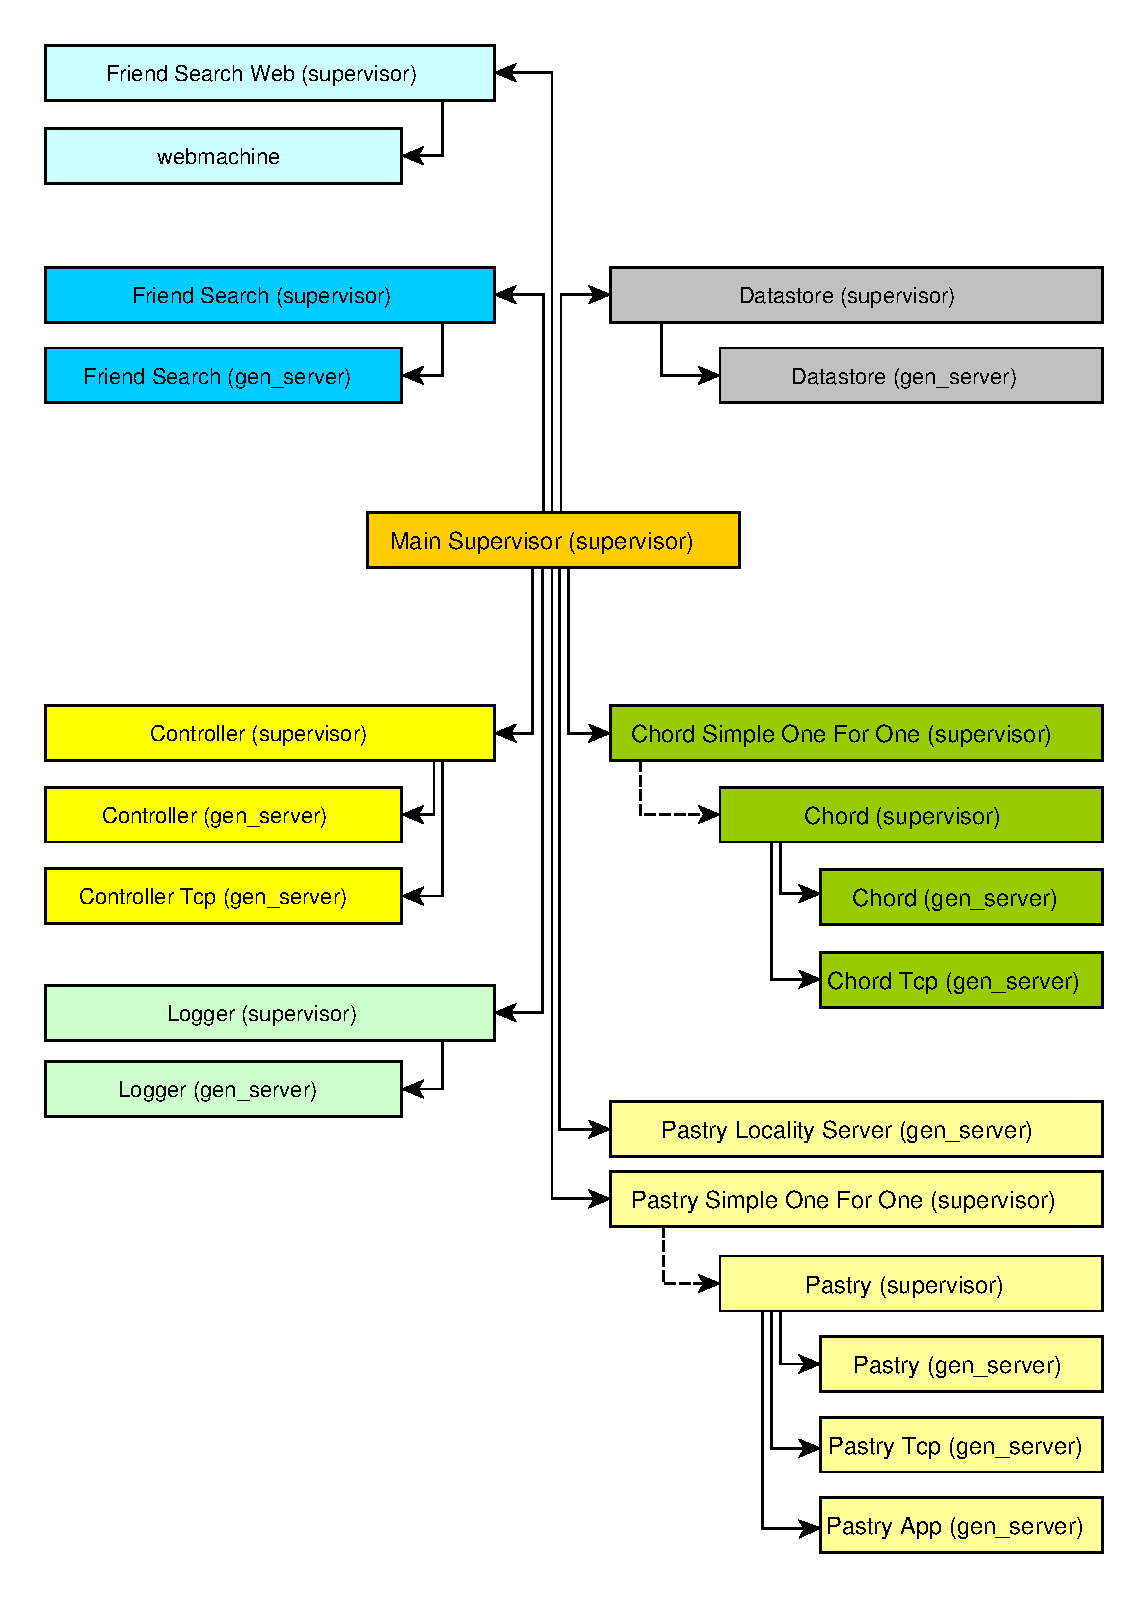
\includegraphics[width=0.9\linewidth]{illustrations/ClientSupervisionTree.eps}
  \caption{This figure shows the hierarchy of supervisors and the servers they supervise.}
  \label{figSupervisionTree}
\end{center}
\end{figure}

Notice how the main supervisor (the box in the middle) supervises a wide range of other supervisors. All of these supervisors, with the exception of the Distributed Hash Table supervisors, in turn supervise a set of servers.

The Chord and Pastry supervisors are a special kind of supervisor. They do not initially start any children, but can be signalled to start and maintain an arbitrary amount of children. This feature allows my system to dynamically adjust the number of Distributed Hash Table nodes that are run at runtime.


\section{Hot code reloading}
The Erlang virtual machine supports hot code reloading.
I built a code distribution service on top of this functionality, that would automatically update the binary code of all running nodes whenever I pushed code changes to my code repository.

This greatly reduced the time it took to change small bugs and experiment with changes after I had deployed my code to a large network of machines.

\mbox{}

In this chapter we have looked at how I developed my system. We looked at high level components and went into details of how routing differs between Chord and Pastry. We then looked at the other central components of my project, the central controlling hub and the search server.

Finally we had a brief look at Erlang supervisors and hot code reloading.
